\begin{frame}
\frametitle{Finite element method}

\begin{itemize}
\item Solve variational equation from 'weak' formulation of the differential equation with bilinear form \(a(u,v)\):
\begin{align*}
\exists u \in V: \forall v \in V: a(u,v) = f(v)
\end{align*}
\item Choose subspace \(V_\text{h}\) with basis \(w_\text{i}\), out of which the approximate solution \(u_\text{h} = \sum u_i w_i \in V_\text{h}\) will be constructed:
\begin{align*}
a(u_\text{h},w_\text{j}) = \sum\limits_i a(w_i,w_\text{j}) \; u_i = f(w_\text{j}) \quad\rightarrow\quad AU = F
\end{align*}
\end{itemize}

\vspace{-0.5em}

\begin{figure}
\hfill{}
\begin{subfigure}{0.2\textwidth}
  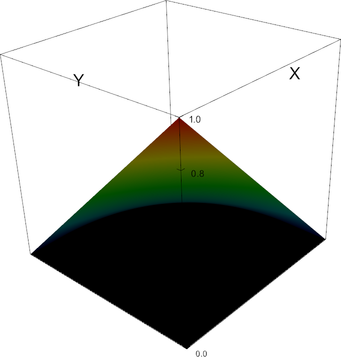
\includegraphics[width=\textwidth]{addendum/figures/Q1_shape0000.png}
\end{subfigure}
\hfill{}
\begin{subfigure}{0.2\textwidth}
  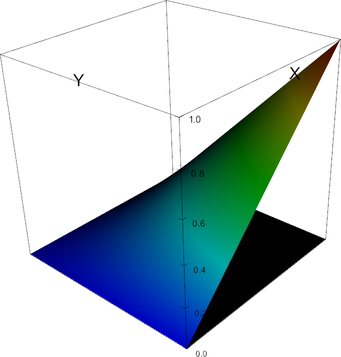
\includegraphics[width=\textwidth]{addendum/figures/Q1_shape0001.png}
\end{subfigure}
\hfill{}
\begin{subfigure}{0.2\textwidth}
  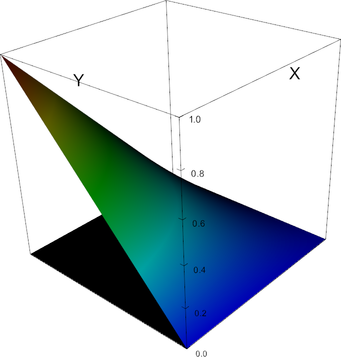
\includegraphics[width=\textwidth]{addendum/figures/Q1_shape0002.png}
\end{subfigure}
\hfill{}
\begin{subfigure}{0.2\textwidth}
  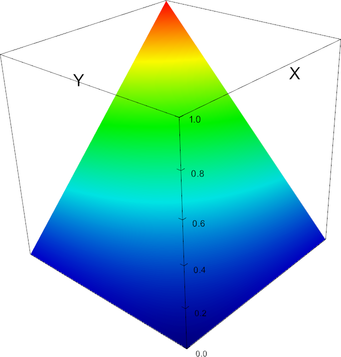
\includegraphics[width=\textwidth]{addendum/figures/Q1_shape0003.png}
\end{subfigure}
\hfill{}
\caption{\(Q_1\) elements in 2D
%  \tiny (source: \href{https://www.dealii.org/8.4.1/doxygen/deal.II/classFE__Q.html}{\underline{deal.II}}) \normalsize
}
\end{figure}
\end{frame}





\begin{frame}
\frametitle{Laplace equation}

Multiply with test function, integrate and apply Gauss theorem
\begin{align*}
- \nabla^2 u &= f \\
- \int_\Omega \nabla^2 u \varphi &= \int_\Omega \nabla u \nabla \varphi - \int_{\partial\Omega} \left(\vectorsym{n} \cdot \nabla\vectorsym{u}\right) \varphi = \int_\Omega f
\end{align*}

$\varphi = 0$ on boundary
\begin{align*}
(\nabla u, \nabla \varphi) &= (f,\varphi)
\end{align*}

Discretized
\begin{align*}
\sum_j \left(\nabla\varphi_i, \nabla \varphi_j \right) u_j &= (f,\varphi_i) \\
AU &= F
\end{align*}
\end{frame}





%\begin{frame}
%\frametitle{Mapping}
%  content...
%\end{frame}





\begin{frame}
\frametitle{Gaussian quadrature}
  
\begin{align*}
  A^K_{ij} &= \int_K \nabla\varphi_i \cdot \nabla \varphi_j \approx \sum_q \nabla\varphi_i(\mathbf x^K_q) \cdot \nabla \varphi_j(\mathbf x^K_q) w_q^K, \\
  F^K_i &= \int_K \varphi_i f \approx \sum_q \varphi_i(\mathbf x^K_q) f(\mathbf x^K_q) w^K_q,
\end{align*}
\end{frame}